%!TeX root = report.tex
%!TEX TS-program = pdflatex

\refstepcounter{chapter}
\addcontentsline{toc}{chapter}{\thechapter\; Эффективные упругие модули пористых и композиционных материалов зернистой структуры}
\begin{center}
{\normalsize\textbf{\centering\thechapter\; ЭФФЕКТИВНЫЕ УПРУГИЕ МОДУЛИ ПОРИСТЫХ И КОМПОЗИЦИОННЫХ МАТЕРИАЛОВ ЗЕРНИСТОЙ СТРУКТУРЫ}}\vspace{14pt} 
\end{center}


%\chapter{Эффективные упругие модули пористых и композиционных материалов зернистой структуры}

\section[Эффективные упругие модули материалов со сферическими порами]{Эффективные упругие модули материалов со сферическими порами\sectionmark{Эффективные упругие модули материалов со сферическими порами}}\sectionmark{Эффективные упругие модули материалов со сферическими порами}

Будем рассматривать пористый материал как упругое пространство $\Omega$ с бесконечной системой сферических полостей $\{\omega_{\alpha\beta\gamma}\}_{\alpha,\beta,\gamma=-\infty}^\infty$, центры которых расположены в узлах $\{O_{\alpha\beta\gamma}\}_{\alpha,\beta,\gamma=-\infty}^\infty$ кубической периодической решетки со стороной $a$. Декартовыми координатами узлов решетки будут упорядоченные наборы чисел $\{(\alpha a,\beta a,\gamma a);\,\alpha,\beta,\gamma\in\mathbb{Z}\}$. Радиусы полостей обозначим через $R$. Выделим отдельную представительскую ячейку пористого материала (рис.~\ref{f:12:1})
$$
\Omega_{\alpha\beta\gamma}=\bigg\{(x_\alpha,y_\beta,z_\gamma): |x_\alpha|\le\dfrac{a}{2},|y_\beta|\le\dfrac{a}{2},|z_\gamma|\le\dfrac{a}{2}\bigg\}.
$$
Здесь ($x_\alpha$, $y_\beta$, $z_\gamma$)~--- локальная декартовая система координат с началом в точке $O_{\alpha\beta\gamma}$.

\begin{figure}[h!]
\centering
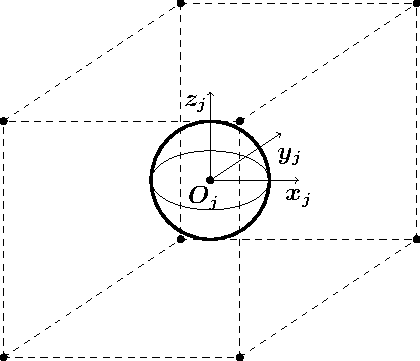
\includegraphics[width=8cm]{cell-spheres.pdf}
\caption{Представительская ячейка пористого материала со сферическими порами}
\label{f:12:1}
\end{figure}

%\begin{equation}
%\begin{cases}
%\dfrac{E_0}{G}\langle\varepsilon_x\rangle+\sigma_0\bigg(\langle\sigma_x\rangle+
%\langle\sigma_z\rangle\bigg)=\langle\sigma_x\rangle, \\
%\dfrac{E_0}{G}\langle\varepsilon_z\rangle+2\sigma_0\langle\sigma_x\rangle=
%\langle\sigma_z\rangle.
%\end{cases}
%\end{equation}

Удельную упругую энергию представительской ячейки можно записать в виде

\begin{equation}
W=\frac{1}{2V}\int\limits_{\Omega_k}\sigma_{ij}\varepsilon_{ij}dv,
\label{eq:12:1}
\end{equation}
где $\Omega_k$~--- представительская ячейка, $V$~--- объем этой ячейки, $\sigma_{ij}$, $\varepsilon_{ij}$~--- компоненты тензоров напряжений и деформаций соответственно. Здесь и далее принято правило суммирования по повторяющимся индексам. Используя формулу Гаусса-Остроградского, объемный интеграл в формуле~\eqref{eq:12:1} можно преобразовать к поверхностному

\begin{equation}
W=\frac{1}{2V}\int\limits_S\sigma_{ij}u_i n_j ds,
\label{eq:12:2}
\end{equation}
где $S$~--- поверхность ячейки $\Omega_k$, $(n_j)_{j=1}^3$~--- направляющие косинусы вектора нормали к поверхности. Заметим, что интеграл по поверхности полости обращается в ноль, так как нормальные напряжения на границе полости равны нулю.
 
В монографии~\cite{Vanin1985} в предположении, что троякопериодичное двухфазное упругое тело находится в однородном поле напряжений, получены два представления удельной энергии деформации через компоненты усредненных напряжений и деформаций в виде

\begin{equation}
W=\frac{1}{2}\langle\sigma_{ij}\rangle\langle\varepsilon_{ij}\rangle,
\label{eq:12:3}
\end{equation}

\begin{equation}
W=\frac{1}{2}c_{ijkl}\langle\sigma_{kl}\rangle\langle\sigma_{ij}\rangle,
\label{eq:12:4}
\end{equation}
где $c_{ijkl}$~--- эффективные упругие постоянные.

Будем использовать результаты задачи упругого деформирования пространства с периодической системой сферических полостей $\Omega\backslash\bigg\{\bigcup\limits_{\alpha,\beta,\gamma}\omega_{\alpha\beta\gamma}\bigg\}$ под действием нагрузки, приложенной на бесконечности (одноосное, двуосное или всестороннее растяжение упругого пространства), приведенные в параграфе 6.1, для вычисления эффективных упругих модулей пористого материала со сферическими порами. В силу того, что на\-пряжен\-но-де\-фор\-ми\-ро\-ван\-ное состояние упругого пространства с периодической системой полостей является однородным, можно считать, что материал с периодической системой пор является изотропным. Как известно, изотропный материал характеризуется двумя независимыми упругими модулями. Для эффективных упругих модулей пористого материала будем использовать следующие обозначения: $K_0$~--- объемный модуль, $E_0$~--- модуль Юнга, $G_0$~--- модуль сдвига, $\sigma_0$~--- коэффициент Пуассона.

При вычислении эффективных упругих модулей используем подход, предложенный в работе~\cite{Vanin1985}.

Пусть упругое пространство с периодической системой полостей подвергается всестороннему растяжению $\sigma_r^\infty=T$, приложенному на бесконечности. При всестороннем растяжении упругого пространства в силу однородности напряженного состояния при вычислении удельной энергии деформации фактически остается одно слагаемое в формуле~\eqref{eq:12:2}

\begin{equation}
W=\frac{1}{2V}\int\limits_S\sigma_{r}u_r ds.
\label{eq:12:5}
\end{equation}
Аналогичная ситуация имеет место в формуле~\eqref{eq:12:3}~\cite{Vanin1985}

\begin{equation}
W=\frac{3}{2}\langle\sigma\rangle\langle\varepsilon\rangle,
\label{eq:12:6}
\end{equation}
где $\langle\sigma\rangle$~--- среднее всестороннее растяжение, $\langle\varepsilon\rangle$~--- средняя деформация рассматриваемого материала при всестороннем растяжении. Приведенные величины связаны соотношением $\langle\sigma\rangle=3K_0\langle\varepsilon\rangle$.

Деформируем представительскую ячейку в равновеликий шар. В данном случае $S$~--- поверхность этого шара. Предполагается, что поверхность $S$ не пересекает границ полостей $\omega_{\alpha\beta\gamma}$. Заменяя под интегралом в формуле~\eqref{eq:12:5} напряжения $\sigma_r$ на средние напряжения
$$
\langle\sigma\rangle=\frac{1}{S}\int\limits_S\sigma_r ds,
$$
с учетом соотношения между средними напряжениями и деформациями получаем формулу для вычисления эффективного объемного модуля

\begin{equation}
K_0=\frac{\langle\sigma\rangle}{\dfrac{1}{V}\int\limits_S u_r ds}.
\label{eq:12:7}
\end{equation}

Вычислим значение интеграла

\begin{equation}
\int\limits_S u_r ds=\int\limits_0^{2\pi}\int\limits_0^\pi u_r R_1^2\sin\theta d\theta d\varphi,
\label{eq:12:8}
\end{equation}
где $R_1$~--- радиус сферы $S$. Для вычисления интеграла~\eqref{eq:12:8} используем результат решения краевой задачи для периодической системы сферических полостей в упругом пространстве~\eqref{eq:11:8s}

\begin{equation}
u_r=\mathbf{U}\cdot\mathbf{e}_r=\mathbf{U}_0\cdot\mathbf{e}_r+\sum\limits_{j=1}^\infty
\sum\limits_{s=1}^3\sum\limits_{n=0}^\infty\sum\limits_{m=-n}^n a_{s,n,m}^{(j)}\mathbf{\tilde U}_{s,n,m}^{+(4)}(r_j,\theta_j,\varphi_j)\cdot\mathbf{e}_r.
\label{eq:12:9}
\end{equation}

Представим перемещения $\mathbf{\tilde U}_{s,n,m}^{+(4)}(r_j,\theta_j,\varphi_j)$ через $\mathbf{\tilde U}_{s,n,m}^{-(4)}(r_1,\theta_1,\varphi_1)$ при помощи теоремы сложения~\eqref{eq:1:99t}.

\begin{multline}
\sum\limits_{j=1}^\infty
\sum\limits_{s=1}^3\sum\limits_{n=0}^\infty\sum\limits_{m=-n}^n a_{s,n,m}\mathbf{\tilde U}_{s,n,m}^{+(4)}(r_j,\theta_j,\varphi_j)= \\
=\sum\limits_{s=1}^3\sum\limits_{n=0}^\infty\sum\limits_{m=-n}^n\bigg\lbrack a_{s,n,m}\mathbf{\tilde U}_{s,n,m}^{+(4)}(r_1,\theta_1,\varphi_1)+ \\
+\mathbf{\tilde U}_{s,n,m}^{-(4)}(r_1,\theta_1,\varphi_1)\sum\limits_{j=2}^\infty\sum\limits_{t=1}^3\sum\limits_{k=0}^\infty\sum\limits_{l=-k}^k a_{t,k,l}\tilde T_{t,k,l,j}^{s,n,m,1}\bigg\rbrack,
\label{eq:12:10}
\end{multline}

Для вычисления $\mathbf{\tilde U}_{s,n,m}^{\pm(4)}\cdot\mathbf{e}_r$ заметим, что
$$
\mathbf{e}_{-1}\cdot\mathbf{e}_r=\frac{1}{2}(\mathbf{e}_x+i\mathbf{e}_y)\cdot(\mathbf{e}_x\sin\theta\cos\varphi+
\mathbf{e}_y\sin\theta\sin\varphi+\mathbf{e}_z\cos\theta)=\frac{1}{2}\sin\theta e^{i\varphi},
$$
$$
\mathbf{e}_1\cdot\mathbf{e}_r=\frac{1}{2}(\mathbf{e}_x-i\mathbf{e}_y)\cdot(\mathbf{e}_x\sin\theta\cos\varphi+
\mathbf{e}_y\sin\theta\sin\varphi+\mathbf{e}_z\cos\theta)=\frac{1}{2}\sin\theta e^{-i\varphi},
$$
$$
\mathbf{e}_0\cdot\mathbf{e}_r=\cos\theta.
$$

Справедливы следующие формулы

\begin{equation}
\mathbf{U}_{1,n,m}^{\pm(4)}\cdot\mathbf{e}_r=-u_{n,m-1}^{\pm(4)}\frac{1}{2}\sin\theta e^{i\varphi}+u_{n,m+1}^{\pm(4)}\frac{1}{2}\sin\theta e^{-i\varphi}\mp u_{n,m}^{\pm(4)}\cos\theta,
\label{eq:12:11}
\end{equation}

\begin{multline}
\mathbf{U}_{2,n,m}^{+(4)}\cdot\mathbf{e}_r=\frac{1}{2n+3}\bigg\{-(n-m+2)(n+m)u_{n,m-1}^{+(4)}\frac{1}{2}\sin\theta e^{i\varphi}+ \\
+(n-m)(n+m+2)u_{n,m+1}^{+(4)}\frac{1}{2}\sin\theta e^{-i\varphi}- \\
-\bigg\lbrack(n-m+1)(n+m+1)+\chi(2n+3)\bigg\rbrack u_{n,m}^{+(4)}\cos\theta+ \\
+(r^2-R^2)\bigg(-u_{n+2,m-1}^{+(4)}\frac{1}{2}\sin\theta e^{i\varphi}+ \\
+u_{n+2,m+1}^{+(4)}\frac{1}{2}\sin\theta e^{-i\varphi}-u_{n+2,m}^{+(4)}\cos\theta\bigg)\bigg\},
\label{eq:12:12}
\end{multline}

\begin{multline}
\mathbf{U}_{2,n,m}^{-(4)}\cdot\mathbf{e}_r=\frac{1}{2n-1}\bigg\{-(n-m+1)(n+m-1)u_{n,m-1}^{-(4)}\frac{1}{2}\sin\theta e^{i\varphi}+ \\
+(n-m-1)(n+m+1)u_{n,m+1}^{-(4)}\frac{1}{2}\sin\theta e^{-i\varphi}+ \\
+\bigg\lbrack(n-m)(n+m)-\chi(2n-1)\bigg\rbrack u_{n,m}^{-4)}\cos\theta+ \\
+(r^2-R^2)\bigg(-u_{n-2,m-1}^{-(4)}\frac{1}{2}\sin\theta e^{i\varphi}+ \\
+u_{n-2,m+1}^{-(4)}\frac{1}{2}\sin\theta e^{-i\varphi}+u_{n-2,m}^{-(4)}\cos\theta\bigg)\bigg\},
\label{eq:12:13}
\end{multline}

\begin{equation}
\mathbf{U}_{3,n,m}^{\pm(4)}\cdot\mathbf{e}_r=u_{n,m-1}^{\pm(4)}\frac{1}{2}\sin\theta e^{i\varphi}+u_{n,m+1}^{\pm(4)}\frac{1}{2}\sin\theta e^{-i\varphi},
\label{eq:12:14}
\end{equation}

Из приведенных формул вытекает

\begin{equation}
\frac{1}{V}\int\limits_S \mathbf{U}_{1,n,m}^{+(4)}\cdot\mathbf{e}_r ds=-\frac{4\pi}{V}\delta_{n1}\delta_{m0},
\label{eq:12:15}
\end{equation}

\begin{equation}
\frac{1}{V}\int\limits_S \mathbf{U}_{2,n,m}^{+(4)}\cdot\mathbf{e}_r ds=-\frac{4\pi(2+\chi)}{3V}\delta_{n1}\delta_{m0},
\label{eq:12:16}
\end{equation}

\begin{equation}
\frac{1}{V}\int\limits_S \mathbf{U}_{3,n,m}^{+(4)}\cdot\mathbf{e}_r ds=0,
\label{eq:12:17}
\end{equation}

\begin{equation}
\frac{1}{V}\int\limits_S \mathbf{U}_{1,n,m}^{-(4)}\cdot\mathbf{e}_r ds=0,
\label{eq:12:18}
\end{equation}

\begin{equation}
\frac{1}{V}\int\limits_S \mathbf{U}_{2,n,m}^{-(4)}\cdot\mathbf{e}_r ds=-\frac{4\pi(-1+\chi)R_1^3}{3V}\delta_{n1}\delta_{m0},
\label{eq:12:19}
\end{equation}

\begin{equation}
\frac{1}{V}\int\limits_S \mathbf{U}_{3,n,m}^{-(4)}\cdot\mathbf{e}_r ds=0.
\label{eq:12:20}
\end{equation}

\begin{equation}
\frac{1}{S}\int\limits_S \mathbf{FU}_{1,n,m}^{+(4)}\cdot\mathbf{e}_r ds=2G\frac{8\pi}{R_1 S}\delta_{n1}\delta_{m0},
\label{eq:12:21}
\end{equation}

\begin{equation}
\frac{1}{S}\int\limits_S \mathbf{FU}_{2,n,m}^{+(4)}\cdot\mathbf{e}_r ds=2G\frac{8\pi(2+\chi)}{3R_1 S}\delta_{n1}\delta_{m0},
\label{eq:12:22}
\end{equation}

\begin{equation}
\frac{1}{S}\int\limits_S \mathbf{FU}_{3,n,m}^{+(4)}\cdot\mathbf{e}_r ds=0,
\label{eq:12:23}
\end{equation}

\begin{equation}
\frac{1}{S}\int\limits_S \mathbf{FU}_{1,n,m}^{-(4)}\cdot\mathbf{e}_r ds=0,
\label{eq:12:24}
\end{equation}

\begin{equation}
\frac{1}{S}\int\limits_S \mathbf{FU}_{2,n,m}^{-(4)}\cdot\mathbf{e}_r ds=-2G\frac{8\pi(1+\sigma)}{3R_1 S}\delta_{n1}\delta_{m0},
\label{eq:12:25}
\end{equation}

\begin{equation}
\frac{1}{S}\int\limits_S \mathbf{FU}_{3,n,m}^{-(4)}\cdot\mathbf{e}_r ds=0,
\label{eq:12:26}
\end{equation}
где $\mathbf{FU}_{s,n,m}^{\pm(4)}$~--- напряжения, отвечающие перемещениям $\mathbf{U}_{s,n,m}^{\pm(4)}$ на поверхности $r_1=R_1$.

Теперь из соотношения~\eqref{eq:12:7} получаем формулу для эффективного объемного модуля

\begin{equation}
\frac{K_0}{K}=\frac{1+\zeta\bigg(2 \tilde a_{1,1,0}+\dfrac{2(5-4\sigma)}{3} \tilde a_{2,1,0}-\dfrac{2(1+\sigma)}{3}\Gamma\bigg)}{1-(1+\sigma)\zeta\bigg(\dfrac{1}{1-2\sigma} \tilde a_{1,1,0}+\dfrac{(5-4\sigma)}{3(1-2\sigma)} \tilde a_{2,1,0}+\dfrac{2}{3}\Gamma\bigg)},
\label{eq:12:27}
\end{equation}
$$
\Gamma=\sum\limits_{t=1}^3\sum\limits_{k=0}^\infty\sum\limits_{l=-k}^k \tilde a_{t,k,l}\sum\limits_{j=2}^\infty\tilde T_{t,k,l,j}^{2,1,0,1},
$$
где $\tilde a_{t,k,l}=\dfrac{2G}{TR^3}a_{t,k,l}$, $a_{t,k,l}$~--- решения линейной системы~\eqref{eq:11:sys}, $\zeta$~--- объемное содержание полостей в материале.

\begin{figure}[h!]
\centering
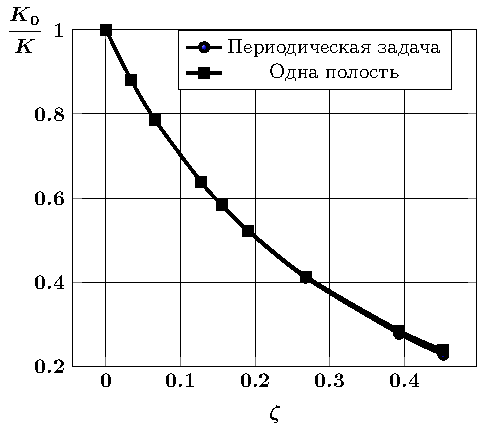
\includegraphics[width=8cm]{porous-spheres-k.pdf}
\caption{Зависимость объемного модуля от объемного содержания полостей в материале}
\label{f:12:2}
\end{figure}

Если решаемую периодическую задачу заменить задачей об определении напряжений и деформаций в упругом пространстве с одной сферической полостью, находящимся под действием всестороннего растяжения, то нужно принять $\Gamma=0$, $\tilde a_{1,1,0}=-1/2$, $\tilde a_{2,1,0}=0$. Тогда формула~\eqref{eq:12:27} превращается в соотношение

\begin{equation}
\frac{K_0}{K}=\frac{(1-\zeta)(2-4\sigma)}{2-4\sigma+(1+\sigma)\zeta},
\label{eq:12:28}
\end{equation}  
которое совпадает с известным результатом, приведенным в монографии~\cite{Vanin1985}.

Таким образом, формула~\eqref{eq:12:27} дает обобщение соотношения~\eqref{eq:12:28}, учитывающее периодическую структуру полостей в материале.

На рис.~\ref{f:12:2} приведены зависимости объемного упругого модуля от объемного содержания полостей в материале. Представлены графики в случаях одной полости в материале и периодической системы полостей в материале. Отличия значений объемных модулей для этих случаев становятся заметными с увеличением объемного содержания полостей. Максимальное отличие достигает 5\% при объемном содержании полостей $\zeta=0.45$. Таким же образом могут быть вычислены остальные эффективные упругие модули.

%***************************************************************************************

\section[Эффективные упругие модули материалов со сферическими включениями]{Эффективные упругие модули материалов со сферическими включениями\sectionmark{Эффективные упругие модули материалов со сферическими включениями}}\sectionmark{Эффективные упругие модули материалов со сферическими включениями}

Будем рассматривать композиционный материал как упругое пространство $\Omega$ с бесконечной системой сферических включений $\{\omega_{\alpha\beta\gamma}\}_{\alpha,\beta,\gamma=-\infty}^\infty$, центры которых расположены в узлах $\{O_{\alpha\beta\gamma}\}_{\alpha,\beta,\gamma=-\infty}^\infty$ кубической периодической решетки со стороной $a$. Декартовыми координатами узлов решетки будут упорядоченные наборы чисел $\{(\alpha a,\beta a,\gamma a);\,\alpha,\beta,\gamma\in\mathbb{Z}\}$. Радиусы включений обозначим через $R$. Считаем, что материалы матрицы и включений имеют упругие постоянные $(\sigma, G)$ и $(\sigma_1, G_1)$. Выделим отдельную представительскую ячейку зернистого композита (рис.~\ref{f:12:1})
$$
\Omega_{\alpha\beta\gamma}=\bigg\{(x_\alpha,y_\beta,z_\gamma): |x_\alpha|\le\dfrac{a}{2},|y_\beta|\le\dfrac{a}{2},|z_\gamma|\le\dfrac{a}{2}\bigg\}.
$$
Здесь ($x_\alpha$, $y_\beta$, $z_\gamma$)~--- локальная декартовая система координат с началом в точке $O_{\alpha\beta\gamma}$. Предполагается, что включения находятся в условиях идеального контакта с матрицей.

%\begin{figure}[h!]
%\centering
%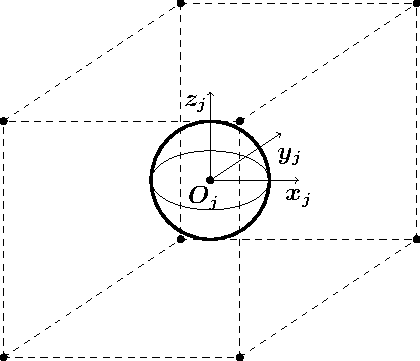
\includegraphics[width=8cm]{cell-spheres.pdf}
%\caption{Представительская ячейка пористого материала со сферическими порами}
%\label{f:12:1}
%\end{figure}

%\begin{equation}
%\begin{cases}
%\dfrac{E_0}{G}\langle\varepsilon_x\rangle+\sigma_0\bigg(\langle\sigma_x\rangle+
%\langle\sigma_z\rangle\bigg)=\langle\sigma_x\rangle, \\
%\dfrac{E_0}{G}\langle\varepsilon_z\rangle+2\sigma_0\langle\sigma_x\rangle=
%\langle\sigma_z\rangle.
%\end{cases}
%\end{equation}

Удельную упругую энергию представительской ячейки можно записать в виде

\begin{equation}
W=\frac{1}{2V}\int\limits_{\Omega_k}\sigma_{ij}\varepsilon_{ij}dv,
\label{eq:12:29}
\end{equation}
где $\Omega_k$~--- представительская ячейка, $V$~--- объем этой ячейки, $\sigma_{ij}$, $\varepsilon_{ij}$~--- компоненты тензоров напряжений и деформаций соответственно. Здесь и далее принято правило суммирования по повторяющимся индексам. Используя формулу Гаусса-Остроградского, объемный интеграл в формуле~\eqref{eq:12:29} можно преобразовать к поверхностному

\begin{equation}
W=\frac{1}{2V}\int\limits_S\sigma_{ij}u_i n_j ds,
\label{eq:12:30}
\end{equation}
где $S$~--- поверхность ячейки $\Omega_k$, $(n_j)_{j=1}^3$~--- направляющие косинусы вектора нормали к поверхности. Заметим, что интеграл по поверхности включения отсутствует в формуле~\eqref{eq:12:30}, так как два таких интеграла для включения и для матрицы взаимно уничтожаются.

При вычислении упругих модулей применим подход, предложенный в монографии~\cite{Vanin1985} и формулы для удельной упругой энергии~\eqref{eq:12:3}, \eqref{eq:12:4}. 

%\begin{equation}
%W=\frac{1}{2}\langle\sigma_{ij}\rangle\langle\varepsilon_{ij}\rangle,
%\label{eq:12:31}
%\end{equation}
%
%\begin{equation}
%W=\frac{1}{2}c_{ijkl}\langle\sigma_{kl}\rangle\langle\sigma_{ij}\rangle,
%\label{eq:12:32}
%\end{equation}
%где $c_{ijkl}$~--- эффективные упругие постоянные.

Будем использовать результаты задачи упругого деформирования пространства с периодической системой сферических включений под действием нагрузки, приложенной на бесконечности (одноосное, двуосное или всестороннее растяжение упругого пространства), приведенные в параграфе 6.2, для вычисления эффективных упругих модулей зернистого композита со сферическими зернами. В силу того, что на\-пряжен\-но-де\-фор\-ми\-ро\-ван\-ное состояние упругого пространства с периодической системой включений является однородным, можно считать, что материал с периодической системой включений является изотропным. Для эффективных упругих модулей композиционного материала будем использовать следующие обозначения: $K_0$~--- объемный модуль, $E_0$~--- модуль Юнга, $G_0$~--- модуль сдвига, $\sigma_0$~--- коэффициент Пуассона.

Пусть упругое пространство с периодической системой включений подвергается всестороннему растяжению $\sigma_r^\infty=T$, приложенному на бесконечности. Повторяя рассуждения предыдущего параграфа, получаем для эффективного объемного модуля формулу

\begin{equation}
\frac{K_0}{K}=\frac{1+\zeta\bigg(2 \tilde a_{1,1,0}+\dfrac{2(5-4\sigma)}{3} \tilde a_{2,1,0}-\dfrac{2(1+\sigma)}{3}\Gamma\bigg)}{1-(1+\sigma)\zeta\bigg(\dfrac{1}{1-2\sigma} \tilde a_{1,1,0}+\dfrac{(5-4\sigma)}{3(1-2\sigma)} \tilde a_{2,1,0}+\dfrac{2}{3}\Gamma\bigg)},
\label{eq:12:31}
\end{equation}
$$
\Gamma=\sum\limits_{t=1}^3\sum\limits_{k=0}^\infty\sum\limits_{l=-k}^k \tilde a_{t,k,l}\sum\limits_{j=2}^\infty\tilde T_{t,k,l,j}^{2,1,0,1},
$$
где $\tilde a_{t,k,l}=\dfrac{2G}{TR^3}a_{t,k,l}$, $a_{t,k,l}$~--- решения линейной системы~\eqref{eq:11:28}, \eqref{eq:11:29}, $\zeta$~--- объемное содержание полостей в материале.

Если решаемую периодическую задачу заменить задачей об определении напряжений и деформаций в упругом пространстве с одним сферическим включением, находящимся под действием всестороннего растяжения, то нужно принять $\Gamma=0$, $\tilde a_{2,1,0}=0$,
$$
\tilde a_{1,1,0}=\frac{G_1(1+\sigma_1)(1-2\sigma)-G(1+\sigma)(1-2\sigma_1)}{(1+\sigma)\bigg\lbrack G_1(1+\sigma_1)+G(2-4\sigma_1)\bigg\rbrack}.
$$
Тогда формула~\eqref{eq:12:31} превращается в соотношение

\begin{multline}
\frac{K_0}{K}=\frac{1-2\sigma}{1+\sigma}\times \\
\times\frac{G(1-2\sigma_1)(1-\zeta)(2+2\sigma)+G_1(1+\sigma_1)(\zeta(2-4\sigma)+1+\sigma)}{G(1-2\sigma_1)(\zeta(1+\sigma)+2-4\sigma)+G_1(1+\sigma_1)(1-\zeta)(1-2\sigma)},
\label{eq:12:32}
\end{multline}  
которое совпадает с известным результатом, приведенным в монографии~\cite{Vanin1985}.

Таким образом, формула~\eqref{eq:12:31} дает обобщение соотношения~\eqref{eq:12:32}, учитывающее периодическую структуру включений в материале.

\begin{figure}[h!]
\centering\footnotesize
\parbox[b]{7.5cm}{\centering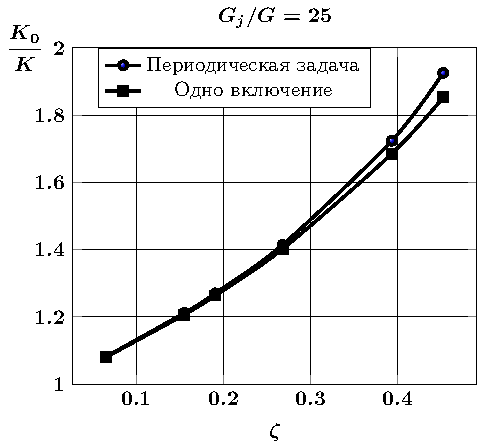
\includegraphics[width=7.5cm]{composite-spheres-g25-k.pdf}
\caption{Зависимость объемного модуля от объемного содержания включений в композите при $G_j/G=25$
\label{f:12:3}}}\hfil\hfil
\parbox[b]{7.5cm}{\centering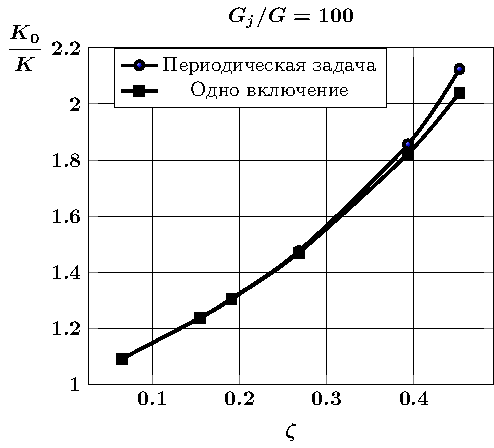
\includegraphics[width=7.5cm]{composite-spheres-g100-k.pdf}
\caption{Зависимость объемного модуля от объемного содержания включений в композите при $G_j/G=100$
\label{f:12:4}}}
\end{figure}

На рис.~\ref{f:12:3}, \ref{f:12:4} приведены зависимости объемного упругого модуля от объемного содержания включений в композиционном материале при $G_j/G=25$ и $G_j/G=100$. Представлены графики в случаях одного включения в материале и периодической системы включений в материале. Отличия значений объемных модулей для этих случаев становятся заметными с увеличением объемного содержания включений. Максимальное отличие достигает 3.5\% при $G_j/G=25$ и 4\% при $G_j/G=100$ в случае объемного содержания включений $\zeta=0.45$. Таким же образом могут быть вычислены остальные эффективные упругие модули.
